\chapter{Planning}

\section{Risk Analysis}

The main purpose of this system will be providing a basic tool for people to test computational model, 

\section{Project Plan}

For this project, I plan to start with understand the how Causcumber work, what kind of result does it produce. Then, following by understand how behave and cucumber function in the system, by understand how these tool works, it would benefit a lot for future plan. The next phase will be designing the user interface for Causcumber, this phase will be focus on design the user interface and making sure it is easy to understand, and easy to operate. After the design the is done, I plan start implement the system, combine the system with the interface, in this phase will be working in Scrum method, where the project will focus on adding or change function based on feedback. The last phase will be polishing the system, focusing on debugging, and making sure the system runs smooth. Below is a graph describing the plan in more detail:

Phase1: Understand how Causcumber work

Phase2: Have a good idea on how behave and cucumber function in Causcumber

Phase3: Design and implement user interface and focus on scrum to gather feedback and \space 

~~~~~~ ~ ~ adjust the system according to it

Phase4: Polish the system and debug or add new function according to feedback if needed

*This schedule is subject to change due to the uncertainty in various phase of the project\\*\\*



\section{Current progress}

This project already has some progress, I already have grasp on how Causcumber work and have move into the scrum phase where a user interface being develop and adding or adjust functions according to feedback, below will be some figure showing the current progress of the system:
\begin{center}
	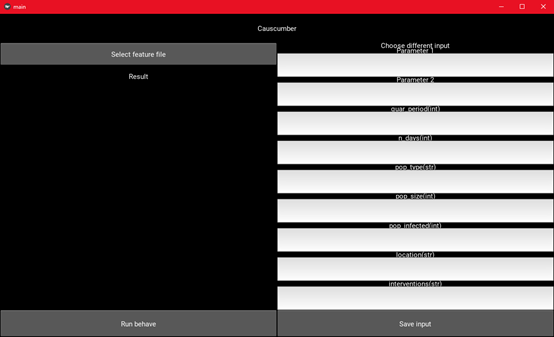
\includegraphics[width=8cm]{figures/Gui_overview.png}\\
	Figure 3. An overview of the user interface
\end{center}
This is an overview of the user interface, the left part will display the result, and the right part is where the users can custom their feature file.
\begin{center}
	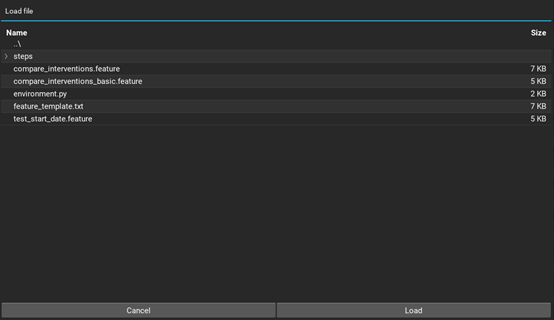
\includegraphics[width=8cm]{figures/select_feature_file.png}\\
	Figure 4. Select feature file screen
\end{center}
User can select which feature file they want to execute, then Causcumber will load and produce the result into a xml file.
\begin{center}
	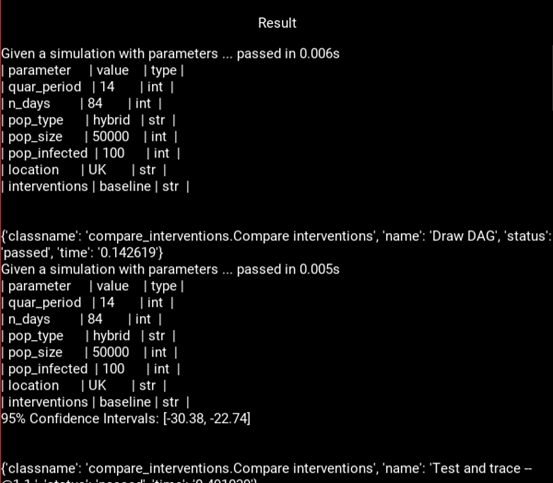
\includegraphics[width=8cm]{figures/Result_display.png}\\
	Figure 5. Result produced by Causcumber and display in the result section
\end{center}
After Causcumber load the feature file and produce to the xml file, the user interface can read from the xml file, retrieve the useful information and remove the unwanted ones, users can view the input parameters and how accurate a parameter in the computational models are.
\begin{center}
	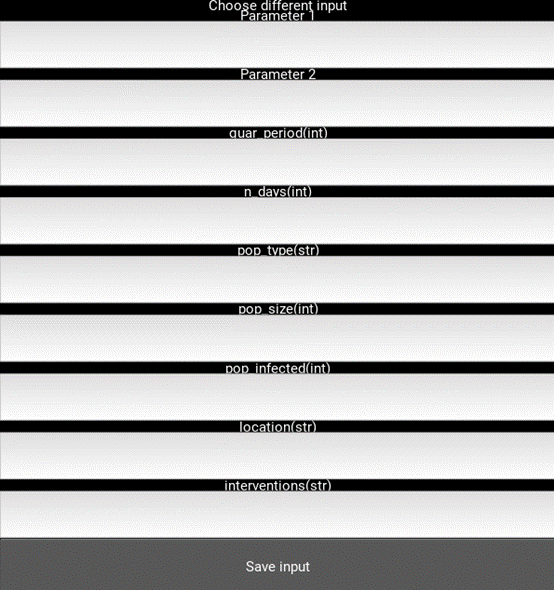
\includegraphics[width=8cm]{figures/Input_section.png}\\
	Figure 6. Choose different input value, and save it into a feature file
\end{center}
In the right side of the interface, user can create their own feature file with their own parameter to test the system, the system will compile the input value and save as a new feature file.
